% !TeX root = ../../../tesis.tex

% =====================================================================
\subsubsection{La Escala Garibelt}
\label{subsubsec:garibelt-escala}
% =====================================================================

El resultado normalizado de cada dimensión cae en algún punto del
intervalo $[0, 1]$. La Escala Garibelt divide ese intervalo en cuatro
bandas que traducen el valor numérico a un diagnóstico territorial.
Crítico $[0.00, 0.25)$ señala una deficiencia estructural severa: la
dimensión requiere intervención antes que cualquier otra. Débil
$[0.25, 0.50)$ indica rendimiento en la mitad inferior del rango de 
referencia normalizada; no constituye una emergencia, pero requiere un plan de mejora. 
Aceptable $[0.50, 0.75)$ describe una dimensión que cumple su función urbana sin
destacar. Idóneo $[0.75, 1.00]$ reserva el extremo superior para redes
con solidez estructural en ese aspecto. La
Figura~\ref{fig:escala-garibelt-barra} muestra la distribución como
espectro continuo.

\begin{figure}[htbp]
\centering
% Diagrama: Escala Garibelt — espectro de 4 bandas
% Usado en: 5-Analisis-Red-Actual/5-6-Clasificacion-Garibelt/5-6-2-Clasificacion.tex
% fig:escala-garibelt-barra
%
% Barra horizontal [0,1] con 4 zonas de color, etiquetas internas,
% valores de corte en la parte inferior y descripción de cada banda.
% Ancho diseñado para \textwidth (≈ 13 cm con márgenes de tesis).

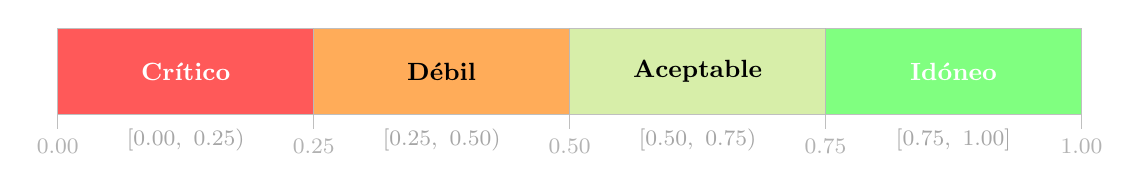
\begin{tikzpicture}

% ================================================================
%  Barra principal — ancho 13 cm, alto 1.1 cm
%  Bandas: 0–3.25 / 3.25–6.50 / 6.50–9.75 / 9.75–13.00
% ================================================================
\fill[red!65]             (0.00, 0) rectangle ( 3.25, 1.10);
\fill[orange!65]          (3.25, 0) rectangle ( 6.50, 1.10);
\fill[yellow!55!green!35] (6.50, 0) rectangle ( 9.75, 1.10);
\fill[green!50]           (9.75, 0) rectangle (13.00, 1.10);
\draw[gray!50, thin]      (0.00, 0) rectangle (13.00, 1.10);
\draw[gray!55, thin] (3.25, 0) -- (3.25, 1.10);
\draw[gray!55, thin] (6.50, 0) -- (6.50, 1.10);
\draw[gray!55, thin] (9.75, 0) -- (9.75, 1.10);

% Etiquetas de banda (centradas en cada zona)
\node[font=\small\bfseries, white]           at (1.625, 0.55) {Crítico};
\node[font=\small\bfseries]                  at (4.875, 0.55) {Débil};
\node[font=\small\bfseries]                  at (8.125, 0.55) {Aceptable};
\node[font=\small\bfseries, white]           at (11.375, 0.55) {Idóneo};

% Rangos numéricos debajo de cada banda
\node[font=\footnotesize, color=gray!70, anchor=north] at (1.625, -0.05)
    {$[0.00,\ 0.25)$};
\node[font=\footnotesize, color=gray!70, anchor=north] at (4.875, -0.05)
    {$[0.25,\ 0.50)$};
\node[font=\footnotesize, color=gray!70, anchor=north] at (8.125, -0.05)
    {$[0.50,\ 0.75)$};
\node[font=\footnotesize, color=gray!70, anchor=north] at (11.375, -0.05)
    {$[0.75,\ 1.00]$};

% Ticks en los puntos de corte
\foreach \xval in {0.00, 3.25, 6.50, 9.75, 13.00}{
    \draw[gray!50] (\xval, 0) -- (\xval, -0.18);
}
\node[font=\footnotesize, color=gray!60, anchor=north] at (0.00,  -0.18) {$0.00$};
\node[font=\footnotesize, color=gray!60, anchor=north] at (3.25,  -0.18) {$0.25$};
\node[font=\footnotesize, color=gray!60, anchor=north] at (6.50,  -0.18) {$0.50$};
\node[font=\footnotesize, color=gray!60, anchor=north] at (9.75,  -0.18) {$0.75$};
\node[font=\footnotesize, color=gray!60, anchor=north] at (13.00, -0.18) {$1.00$};

\end{tikzpicture}

\caption[Escala Garibelt: espectro de cuatro bandas de diagnóstico]{%
    Escala Garibelt: distribución del intervalo $[0,1]$ en cuatro bandas
    de diagnóstico territorial. Cada dimensión del Espectro MJG recibe
    una banda según su valor normalizado.}
\label{fig:escala-garibelt-barra}
\fuentefigura{Elaboración propia.}
\end{figure}

% =====================================================================
\subsubsection{Qué pregunta responde cada dimensión}
\label{subsubsec:garibelt-preguntas}
% =====================================================================

Para leer el Espectro MJG sin necesidad de conocer los detalles
computacionales, conviene tener presente qué pregunta urbana responde
cada dimensión:
\begin{itemize}
    \item Cobertura~$C$: ¿cuánto del área metropolitana queda dentro del
          radio de caminata de la red?
    \item Fuerza capilar~$C_i$: ¿qué tan variadas son las opciones de
          conexión disponibles en cada nodo?
    \item Índice de ruta directa~$DI$: ¿obliga la red a recorrer
          trayectos muy alejados de la distancia mínima?
    \item Tiempo promedio~$T$: ¿cuánto dura un viaje típico de extremo
          a extremo de la red?
    \item Intermediación~$B(v)$: ¿depende el flujo de la red de unos
          pocos nodos críticos o está distribuido entre muchos?
\end{itemize}
Cada banda del Espectro se lee como la respuesta a esa pregunta: Crítico
significa que la respuesta es desfavorable en grado severo; Idóneo,
que la red cumple con solidez estructural en esa dimensión.

% =====================================================================
\subsubsection{El procedimiento de normalización}
\label{subsubsec:garibelt-procedimiento}
% =====================================================================

Llevar un valor bruto a la escala $[0, 1]$ de la Clasificación Garibelt
requiere un rango de referencia. Para~$T$, ese rango lo entrega la
\textsc{enoe}: los tiempos de traslado en la \cdmx{} oscilan en la
práctica entre 85 y 180 minutos, de modo que 85 min normaliza a $1.0$
(Idóneo) y 180 min a $0.0$ (Crítico). Para~$DI$, la teoría de grafos
fija el piso en $1.0$ ---ruta directa perfecta--- y la práctica urbana
establece el techo en $2.5$ ---desviación que ya resulta inaceptable
para el usuario. Para~$C$, el estándar peatonal urbano de 80\,\% es la
referencia. Para~$C_i$, el rango es el del propio dataset: los
percentiles Q1 y Q3 de la distribución de grado nodal. Para~$B(v)$,
se calcula el índice de Gini de la distribución completa de
intermediación y se invierte: Gini~$= 0$ (distribución perfecta) da
$1.0$; Gini cercano a $1$ (monopolio) da $0.0$. La
la Tabla~\ref{tab:clasificacion-garibelt-dims} consolida estos rangos.

% =====================================================================
\subsubsection{Un tablero, no un marcador}
\label{subsubsec:garibelt-tablero}
% =====================================================================

Una ciudad puede cubrir la cuota legal de suministro de agua y tener,
al mismo tiempo, colonias con presión insuficiente, cortes en horas punta
y parámetros de saneamiento fuera de norma. Un clasificador escalar único
---«porcentaje de cobertura hídrica»--- tendería a ocultar esos puntos de
falla detrás de un valor promedio que parece satisfactorio. El transporte
metropolitano enfrenta el mismo problema de escala: la red puede mostrar
tiempos de viaje razonables y, en paralelo, tener toda su carga
concentrada en dos o tres nodos que la vuelven estructuralmente frágil.
La Clasificación Garibelt mantiene las cinco dimensiones separadas
precisamente para no perder esa información. \citet{deng2023} articulan
el principio como \termino{Safe-to-Fail}: evaluar una red es localizar
sus vulnerabilidades, no suavizarlas en un promedio. La subsección
siguiente presenta el procedimiento con un ejemplo hipotético.
